\documentclass[../../thesis.tex]{subfiles}

\begin{document}

\TODO{relate our work to TimeVQVAE, Neural Representation, Barlow, MaskGIT, }

\TODO{Include something on time series generation / representation learning}



% To our knowledge the joint embedding VQ-VAE models presented in this thesis are new.

\section{TimeVQVAE}

TimeVQVAE is a time series generation model based on VQVAE and MaskGIT. It is the first to our and the authors knowledge that utilizes vector quantization (VQ) to address the TSG problem. It leverages a two stage approach similar to VQVAE and uses a bidirectional transformer akin to MaskGIT for prior learning. Additionally, they propose VQ modeling in time-frequency domain, separating data into high and low frequency components to better retain temporal consistencies and generate higher quality samples.\newline

TimeVQVAE provides class-guided conditional sampling.

Our work in this thesis can be seen as a tangent of the paper "Vector Quantized Time Series Generation with a Bidirectional Prior Model" \cite{TimeVQVAE}. We simplify the architecture by omitting the HF/LF split. This reduces prior learning to resemble MaskGIT to a larger degree. 

% The TimeVQVAE model based on \cite{VQVAE} and is a two staged process. The TimeVQVAE model adressed some shortcomings of the VQVAE model when applied to time series data, most notably its inability/difficulty to generate/reconstruct high frequency components. In particular they train the quantizer on the time-frequency representation of the time series using the short time fourier transform and handle the high and low frequency components separately. \newline
% For prior learning TimeVQVAE uses a bi-directional transformer akin to \cite{chang2022maskgit}, but modified to handle the two modalities HF and LF.  \newline

\subsection{Tokenization}

\subsection{Prior learning}

\section{MaskGIT}

The Masked Generative Image Transformer (MaskGIT) is a generative transformer model for image synthesis developed by Google Research. The novelty of the model lies in the token generation. Unlike popular autoregressive generative transformers, who treat images as a sequence of tokens, MaskGIT introduces an image synthesis paradigm using a bi-directional transformer decoder. This means that during training MaskGIT learns to predict tokens in all directions, an intuitively more natural way to consider images. At inference time MaskGIT starts out with a blank canvas and predicts the entire image, and iteratively keeps and conditions on the most confident pixels.\newline

The model assumes a tokenization procedure for stage 1, and in the original paper they used VQGAN \cite{VQGAN}. As MaskGIT only focuses on improving stage 2, present only that part. 

\subsection{Masked Visual Token Modeling (Prior learning)}

For some image $X$ in the dataset $\mathcal{D}$, let $Y = \{y_i\}_{i=1}^N$ denote the latent tokens obtained by passing $X$ through the VQ-Encoder and denote the corresponding binary mask by $M = \{m_i\}_{i=1}^N$. During training a subset of $Y$ is replaced by a special masking token we denote by $\M$ according to the binary mask $M$. This is done by 

\begin{equation}
    Y_\text{Mask} = Y\odot (1_N-M) +  M\cdot\M,
\end{equation}

where $\odot$ is the Hadamard product, i.e point wise multiplication, and $1_N$ is a vector with the same shape as $M$ and $Y$.\newline

The sampling procedure, or choice number of tokens to mask, is parameterized by a mask scheduling function $\gamma$. The sampling can be summarized as follows

\begin{itemize}
    \item Sample $r \sim U(0,1]$.
    \item Sample $\lceil \gamma(r)\cdot N \rceil$ indices $I$ uniformly from $\{0,\dots,N-1\}$ without replacement. 
    \item Create $M$ by setting $m_i = 1$ if $i\in I$, and $m_i = 0$ otherwise.
\end{itemize}

The training objective is to minimize the negative log likelihood of the masked tokes, conditional on the unmasked

\begin{equation}
    \loss_\text{Mask} = -\E_{Y\in \mathcal{D}}\left[\sum_{i \in I} p(y_i|Y_\text{Mask} ) \right]
\end{equation}

\begin{figure}[h]
    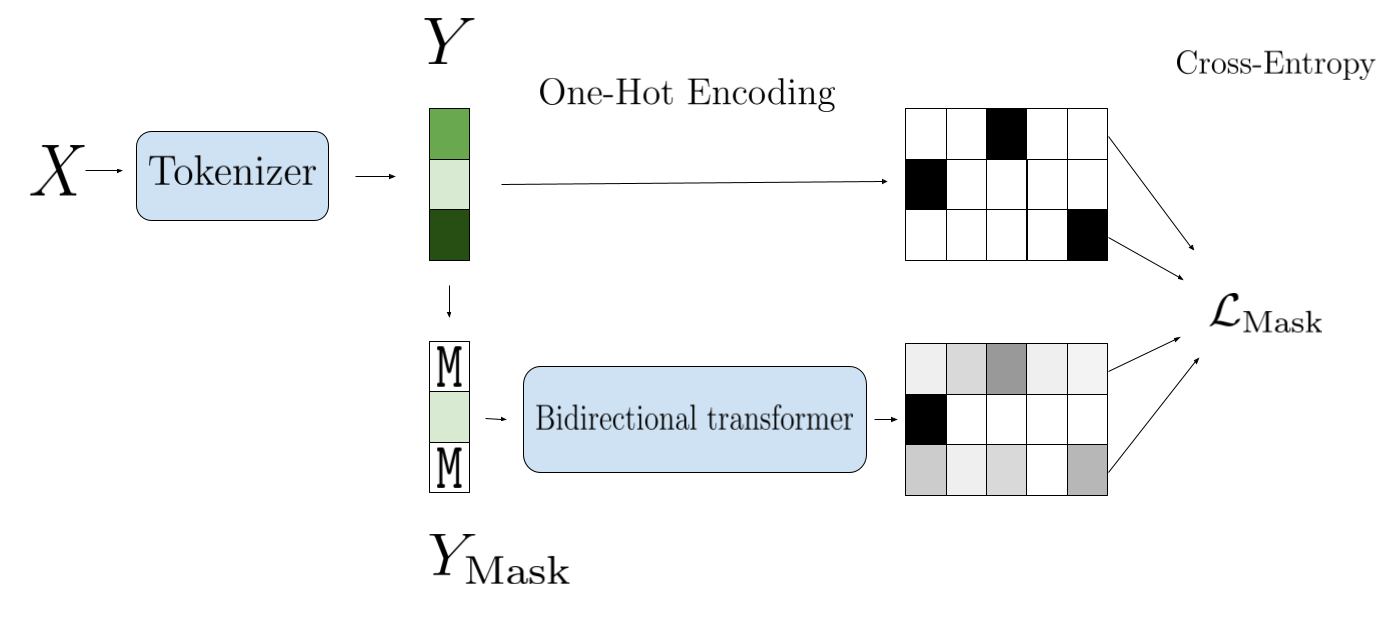
\includegraphics[scale=0.23]{MaskGIT.png}
    \centering 
    \label{fig:MaskGIT}
    \caption{MaskGIT forward computation.}
\end{figure}

A bidirectional transformer is used to predict the probabilities $p(y_i|Y_\text{Mask})$ of each masked token, and $\loss_\text{Mask}$ is computed as the cross entropy between the ground truth one-hot token and the predicted token.




% Start out with a sequence $s$ (b,n) of codebook indices corresponding to a discrete latent representation $z_q$. Determine the proportion of tokens to mask according to the mask scheduling function $\gamma(t)\in (0,1]$. 
% Sample a random subset of $s$ and replace values by [MASK] token in order to create the masked sequence $s_M$ (b,n). By a forward pass of the bi-directional transformer with $s_M$ as input obtain unnormalized logits (b,n,K), defining a distribution over the codebook indices at each element. Calculate the loss as the binary cross-entropy of the logits and $s$. 

\subsection{Iterative decoding (Image generation)}

The bi-directional transformer could in principle predict all $\M$ tokens and generate a sample in a single pass by simply sampling from the predicted probabilites $p(y_i|Y_\text{Mask})$ from a forward pass of an all masked sequence. However, there are challenges with this approach. In their original article \cite{chang2022maskgit} proposes a novel non-autoregressive decoding method to sythesize samples in a constant number of steps.\newline

The decoding process goes from $t = 0$ to $T$. To generate a sample at inference time one starts out with a all masked sequence which we denote by $Y_\text{Mask}^{(0)}$. At iteration $t$ the model predicts the probabilities for all the mask tokens, $p(y_i|Y_\text{Mask}^{(t)})$, in parallel. At each masked index $i$ a token $y_i^{(t)}$ is sampled according to the predicted distribution, and the corresponding probability $c_i^{(t)}$ is used as a measure of the confidence in the sample. For the unmasked tokens a confidence of $1$ is assigned to the true position. The number of $y_i^{(0)}$ with highest confidence kept for the next iteration is determined by the mask scheduling function. We mask $n = \lceil \gamma(t/T)\cdot N \rceil$ of the lower confidence tokens by calculating $M^{(t+1)}$ by 

\begin{equation}
    m_i^{(t+1)} = 
    \begin{cases}
        1, \text{ if } c_i < \text{Sort}([c_1^{(t)},\dots,c_N^{(t)}])[n]\\
        0, \text{ otherwise} 
    \end{cases}
\end{equation}
\begin{figure}[h]
    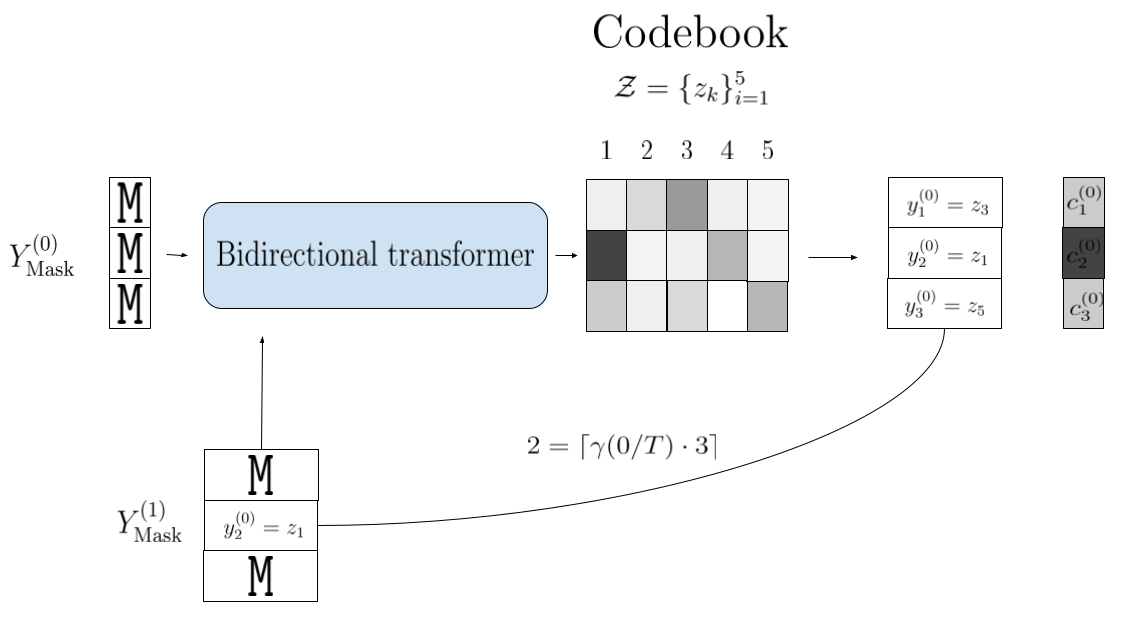
\includegraphics[scale=0.35 ]{IterativeDecoding.png}
    \centering 
    \label{fig:IterativeDecoding}
    \caption{Illustration of first pass of the iterative decoding algorithm.}
\end{figure}

The algorithm synthesizes a full image in $T$ steps.  


\subsection{Masking design}

For image generation, cosine scheduling function proved best across all experiments in the original paper. Start out by selecting just a few 




\section{SSL}

Our model leverages SSL algorithms in order to learn more expressive latent representations. Here we present the relevant algorithms for our work. 

% \subsection{BYOL}
% \cite{grill2020bootstrap}
% Bootstrap Your Own Latents (BYOL) is an early non-contrastive self supervised learning algorithm developed by Google Research in 2020. BYOL was developed for image representation learning and provided a new state of the art for downstream classification accuracy on ImageNet using a linear evaluation with a ResNet-50 architecture. 

% How it works:
% BYOL uses a joint embedding architecture, one \textit{online} network and a \textit{target} network. Both networks consists of an encoder $f$ and decoder $g$, while the online network too has a predictor $q$. The architecture of the networks are the same, but the target parameters $\zeta$ are exponential moving averages of the online parameters $\theta$. In particular, for a specified target decay rate $\tau\in[0,1]$, the target parameters are updated according to 
% \begin{equation}
%     \zeta \leftarrow \tau \zeta + (1-\tau)\theta
% \end{equation}
% after each training step. \\\\

% Let $\mathcal{D}$ be the data. As is typical for non contrastice SSL, data augmentations are applied in order to increase robustness of the representations. Let $\mathcal{T}$  and $\mathcal{T'}$ denote the set of augmentations for the online and target network respectively. BYOL samples a data point $x\sim \mathcal{D}$ and two augmentation $t\sim \mathcal{T}$ and $t'\sim \mathcal{T'}$, with whom it creates two views $v = t(x)$ and $v' = t'(x)$. The views maps through their respective branch as follows
% \begin{equation}
%     x \to t(x) = v \to f_\theta(v) = y_\theta \to g_\theta (y_\theta) = z_\theta \to p_\theta(z_\theta)
% \end{equation}
% \begin{equation}
%     x \to t'(x) = v' \to f_\zeta(v') = y'_\zeta \to g_\zeta (y'_\zeta) = z'_\zeta,
% \end{equation}
% and both outputs are $l_2$-normalized before their mean squared error is calculated. In other words the outputs are updated as
% \begin{equation}
%     \bar{p}_\theta(z_\theta) = \frac{p_\theta(z_\theta)}{||p_\theta(z_\theta)||_2}, \quad \bar{z}_\zeta' = \frac{z_\zeta'}{||z_\zeta'||_2},
% \end{equation}
% before the loss is obtained by 
% \begin{equation}
%     \mathcal{L}_{\theta,\zeta} = ||\bar{p}_\theta(z_\theta) - \bar{z}_\zeta'||_2^2 = 2-2 \frac{\langle p_\theta(z_\theta), z_\zeta'\rangle}{||p_\theta(z_\theta)||_2\cdot||z_\zeta'||_2}
% \end{equation}

% The BYOL loss is obtain by symmetrizing $\mathcal{L}_{\theta,\zeta}$. This is done by separately feeding $v'$ into the online network and $v$ into the target network, and calculating $\mathcal{\tilde{L}}_{\theta,\zeta}$ to obtain $\mathcal{L}^{\text{BYOL}}_{\theta,\zeta} = \mathcal{L}_{\theta,\zeta} + \mathcal{\tilde{L}}_{\theta,\zeta}$


% \TODO{Figure}



\subsection{Barlow Twins}
What is it?

Barlow Twins is a non-constrastive SSL method based on applying the \textit{redundancy-reduction principle} (or efficient coding hypothesis) \cite{Barlow_origin} from the neroscientist H. Barlow to a pair of identical networks. 

In essence the models encurage representations of similar samples to be similar, while simultaneously reducing the amount of redundancy between the components of the vectors. This is done by producing two distorted views of each sample and embedding these in a vast feature space, in such a way that their cross-correlation is close to the identity. 

How does it work?

Start out with a sample $X$ and creates two augmented (distorted) views $X_1$ and $X_2$. The views are then mapped to a latent space by two identical encoders, giving $Y_1$ and $Y_2$. Then the projector embeds the latent representations in a vast space, giving $Z_1$ and $Z_2$. Finally the similarity of the two embeddings are measured by the empirical cross-corelation.

\TODO{Ask for premission?? to use this or make own}
\begin{figure}[h]
    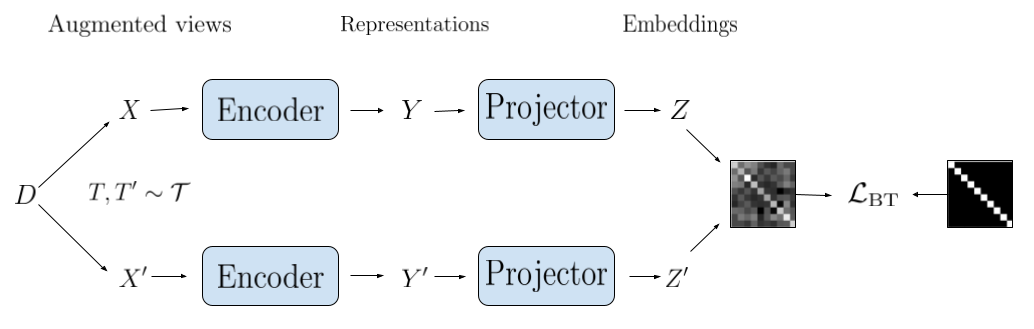
\includegraphics[scale=0.2]{BarlowTwins.png}
    \centering    
    \caption{\cite{zbontar2021barlow}}
\end{figure}

The loss function is calculated as the difference of the empirical cross-correlations of $Z_1$ and $Z_2$ is then calculated and the identiry matrix. 


\subsection{VIbCReg}
\TODO{What is it?}

VIbCReg \cite{lee2024vibcreg} is a non-contrastive SSL model based on VICReg \cite{bardes2022vicreg}, but with better covariance regularization.  It has a joint embedding architecture. 

\TODO{How it works}
Two different views of the input data is encoded into representations $Y$ $Y'$. The representations are further mapped to a larger space by a \textit{projector} with an IterNorm \cite{huang2019iterative} layer. The loss is computed using the projected values $Z$ and $Z'$. \newline
The loss consists of a similarity loss between the branches, and feature decoration (FD) loss together with a feature component expressiveness (FcE) term at each branch. 

\TODO{Loss}
Input data is processed in batches. Denote $Z = [z_1,...,z_B]^T \in \mathbb{R}^{B\times F}$, and similarly for $Z'$, where $B$ and $F$ denotes the batch and feature sizes respectively. $\text{Var}()$ is a variance estimator, $\gamma$ is a target value for the standard deviation, which both in VIbCReg and VICReg is set to $1$. $\epsilon$ is a small scalar preventing numerical instabilities.\newline 
Similarity loss

\begin{equation}
    s(Z,Z') = \frac{1}{B} \sum_{b=1}^B || Z_b-Z_b'||_2^2
\end{equation}

FcE/Variance term

% \begin{equation}
%     v(z) =  \frac{1}{F} \sum_{f=1}^F \max(0,\gamma - \sqrt{\text{Var}(Z_f)+\epsilon})
% \end{equation}


FD/covariance term

\begin{equation}
    C(Z) = \frac{1}{B-1} \left(\frac{Z-\bar{Z}}{||Z-\bar{Z}||_2}\right)^T\left(\frac{Z-\bar{Z}}{||Z-\bar{Z}||_2}\right) \text{ where }  \bar{Z} = \sum_{b=1}^B  Z_b
\end{equation}

% \TODO{Ask Daeso if i can use image}
% \begin{figure}[h]
%     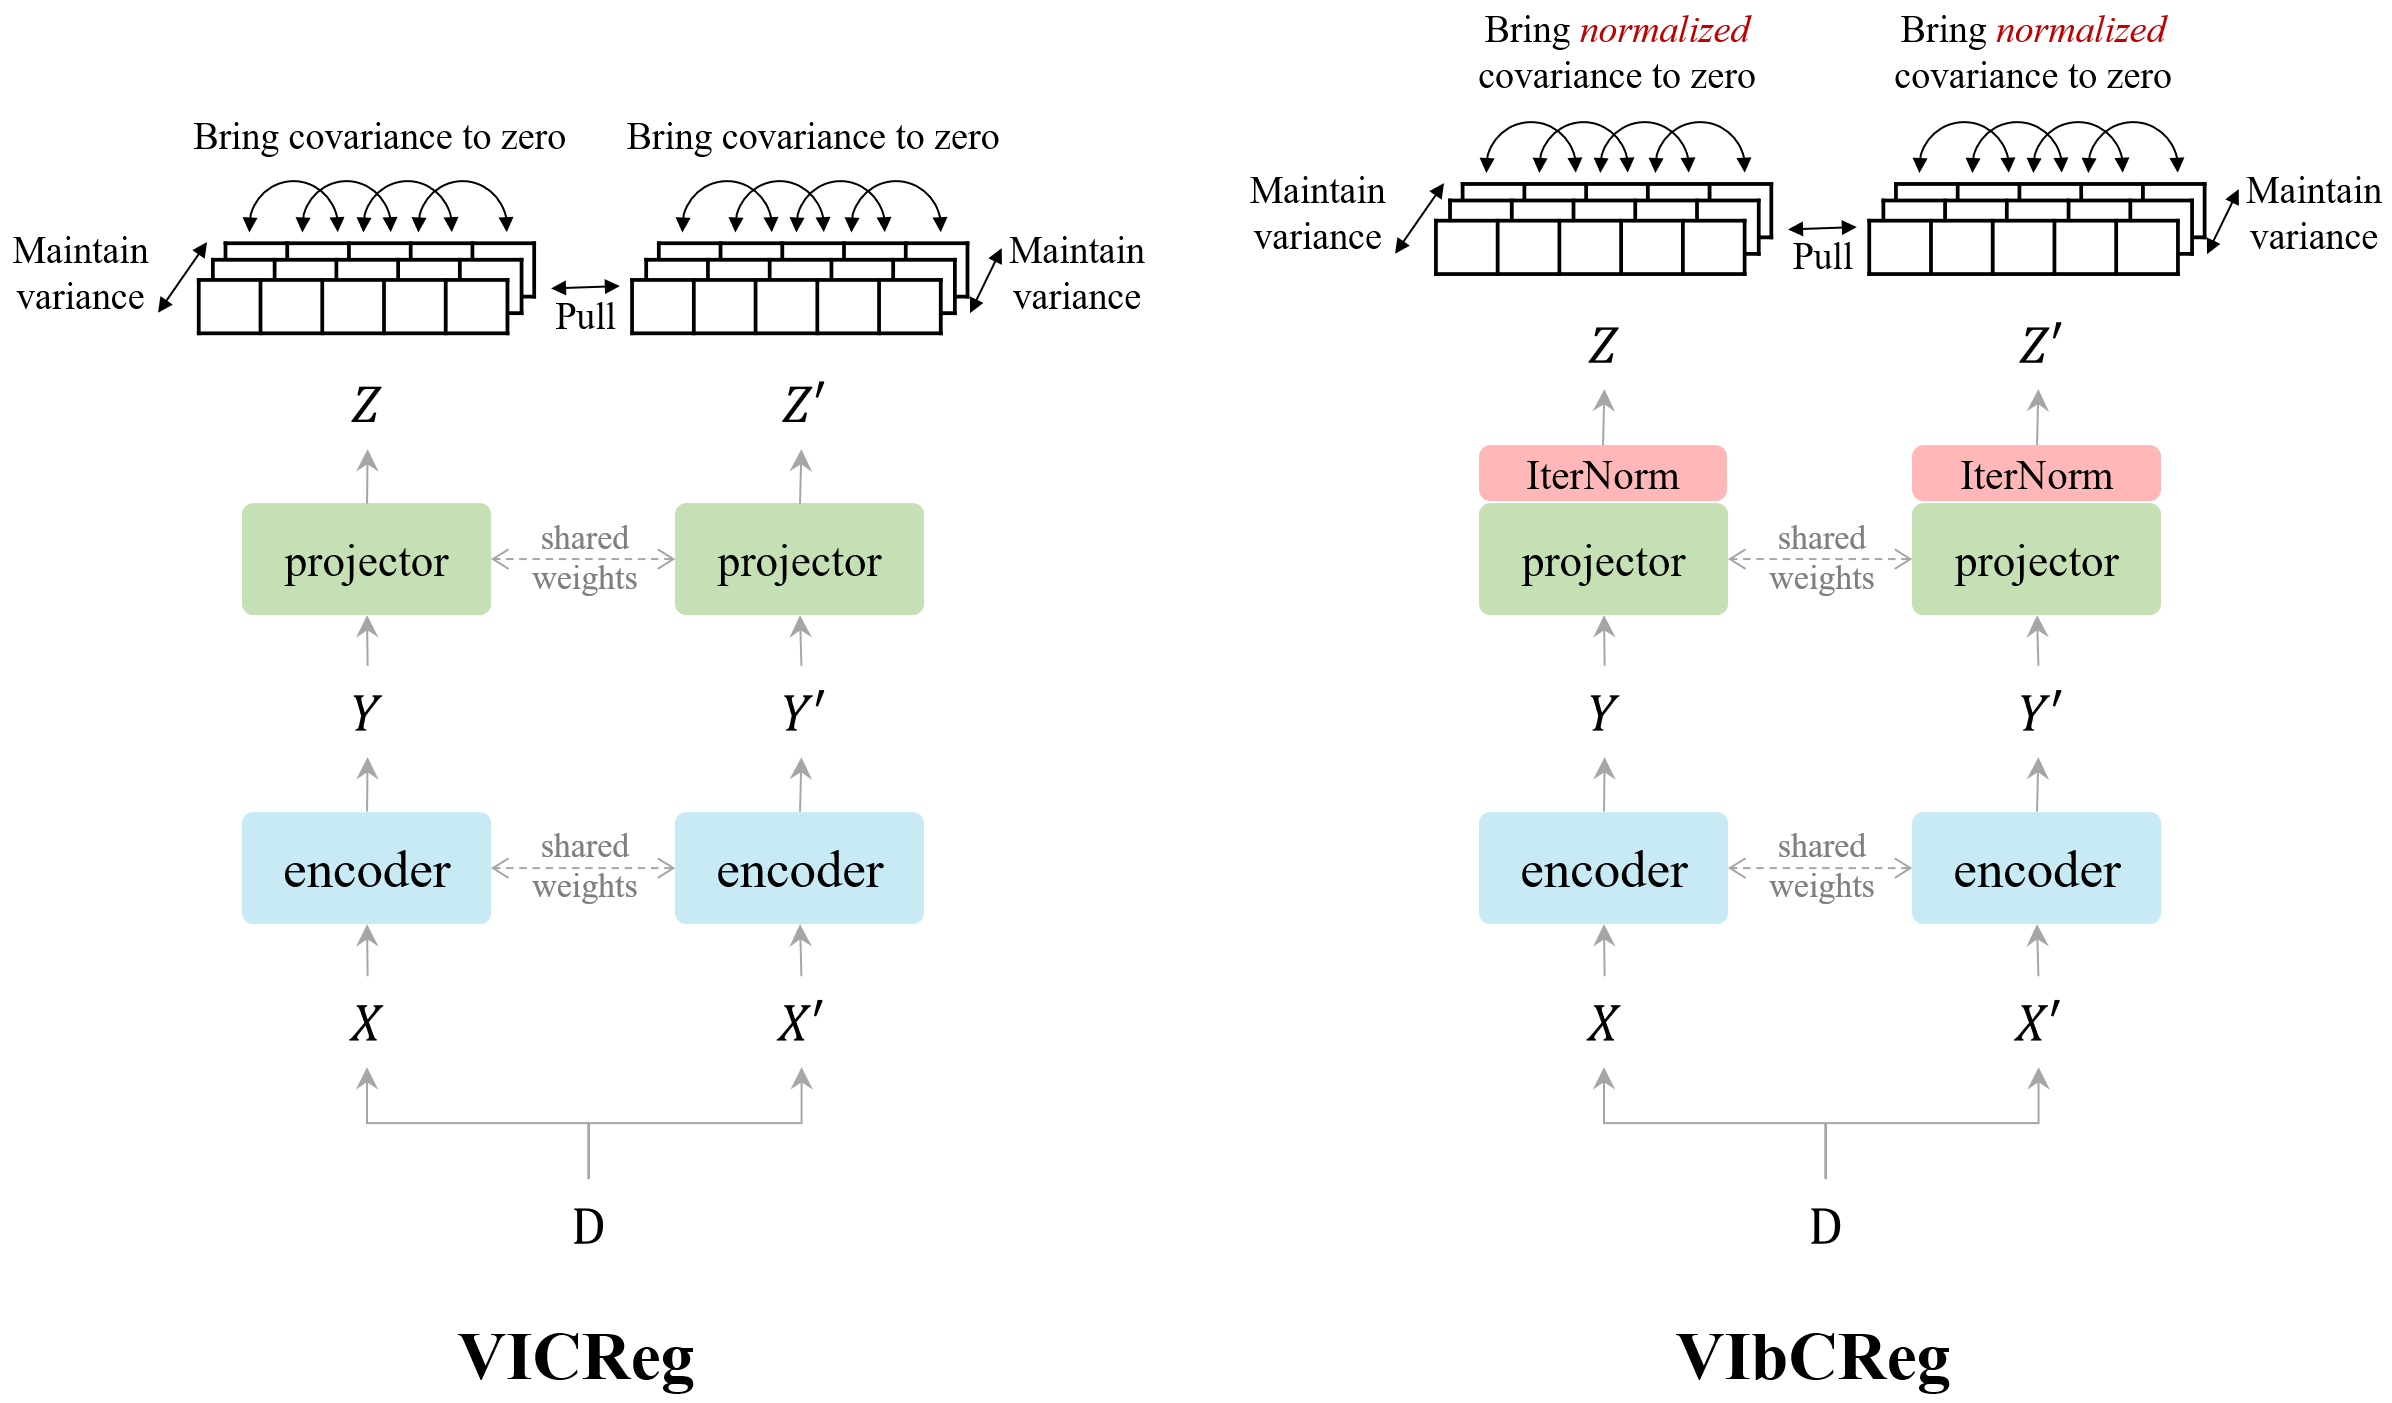
\includegraphics[scale=0.15]{VICReg_VIbCReg.png}
%     \centering    
%     \caption{\cite{lee2024vibcreg}}
% \end{figure}




\end{document}